\begin{table}[t!]
    \small
    \centering
    \begin{tabular}[width=\linewidth]{l|c|c|c|c}
    \hline
    ~               & input        & \#views    & accuracy & accuracy \\ 
    ~ & & & avg. class & overall \\ \hline
    SPH~\cite{kazhdan2003rotation}             & mesh        & - & 68.2         & -  \\ \hline
    3DShapeNets~\cite{wu20153d}     & volume       & 1        & 77.3  & 84.7 \\
    VoxNet~\cite{maturana2015voxnet}          & volume       & 12        & 83.0 & 85.9 \\
    Subvolume~\cite{qi2016volumetric}    & volume       & 20      & 86.0  & \textbf{89.2} \\ \hline
    LFD~\cite{wu20153d}             & image        & 10        & 75.5 & -\\
    MVCNN~\cite{su15mvcnn}           & image        & 80        & \textbf{90.1} & -\\ \hline
    Ours baseline  & point    & -     & 72.6  & 77.4\\
    Ours PointNet   & point   & 1        & 86.2 & \textbf{89.2} \\ \hline
    \end{tabular}
    \caption{\textbf{ModelNet40上的分类结果} 我们的网络在一系列3D输入的深度网络中达到最先进的效果。}
    \label{tab:classification}
\end{table}
\label{sec:exp}
实验被分成了四部分。首先,我们展示了PointNets可以应用于多个3D识别任务 (Sec~\ref{sec:application})。 其次,我们提供了详细的实验来验证我们的网络设计 (Sec~\ref{sec:arch_analysis})。最后,我们可视化了网络学到的内容 (Sec~\ref{sec:visualizing_pointnet}) 并且分析了时间和空间复杂度 (Sec~\ref{sec:complexity})。



\begin{table*}[th!]
    \small
    \centering
    \begin{tabular}[width=\linewidth]{l|c|p{0.5cm}p{0.4cm}p{0.4cm}p{0.4cm}p{0.5cm}p{0.6cm}p{0.5cm}p{0.5cm}p{0.5cm}p{0.6cm}p{0.6cm}p{0.3cm}p{0.5cm}p{0.6cm}p{0.6cm}p{0.6cm}}
    \hline
    ~        & mean & aero & bag & cap & car & chair & ear & guitar & knife & lamp & laptop & motor & mug & pistol & rocket & skate & table \\ 
    &   & &  &  &  &  & phone &  &   &  &  & &    &    &    & board &  \\ \hline
    \# shapes & & 2690 & 76 & 55 & 898 & 3758 & 69 & 787 & 392 & 1547 & 451 & 202 & 184 & 283 & 66 & 152 & 5271 \\ \hline
    Wu~\cite{Wu2014248} &  -  & 63.2  & - &      -    & -   & 73.5 & - &    - &    - &     74.4  & -    & - &   -   &   -   &   - & -  &  74.8 \\
    Yi~\cite{Yi16} & 81.4 & 81.0 & 78.4 & 77.7 & \textbf{75.7} & 87.6 & 61.9 & \textbf{92.0} & 85.4 & \textbf{82.5} & \textbf{95.7} & \textbf{70.6} & 91.9 & \textbf{85.9} & 53.1 & 69.8 & 75.3 \\ \hline
    3DCNN & 79.4 & 75.1 & 72.8 & 73.3 & 70.0 & 87.2 & 63.5 & 88.4 & 79.6 & 74.4 & 93.9 & 58.7 & 91.8 & 76.4 & 51.2 & 65.3 & 77.1 \\ 
    Ours & \textbf{83.7} & \textbf{83.4} & \textbf{78.7} & \textbf{82.5} & 74.9 & \textbf{89.6} & \textbf{73.0} & 91.5 & \textbf{85.9} & 80.8 & 95.3 & 65.2 & \textbf{93.0} & 81.2 & \textbf{57.9} & \textbf{72.8} & \textbf{80.6} \\ \hline
    \end{tabular}
    \caption{\textbf{ShapeNet数据集上的分割结果} 评价指标是点集的mIoU(\%)。 我们与两种传统方法 \cite{Wu2014248} \cite{Wu2014248} 以及我们提出的三维卷积网络对比。PointNet方法在mIoU上达到最佳表现。}
    %Notice that while all the other three methods are tested on the official ShapeNet train/validation/test split~\cite{shapenet2015}, the statistics for Wu's method~\cite{Wu2014248} are tested on a much larger set of shapes.
    \label{tab:segmentation}
\end{table*}



\subsection{应用}
\label{sec:application}
在本节中,我们将展示我们的网络是如何经过训练,来完成3D目标分类、目标零件分割和场景语义分割任务\footnote{更多应用样例,例如形状对应和基于点云的CAD模型检索包含在补充资料中。} 即使我们基于全新的数据表示(点集)进行研究,我们也能够在多个任务的基准测试中获得相当的甚至更好的性能。

\paragraph{3D目标分类} 我们的网络学习了可用于目标分类的全局点云特征。我们在ModelNet40~\cite{wu20153d} 形状分类基准上评估了我们的模型。总共有来自40个人造目标类别的12311个CAD模型,分为用于训练的9843个和用于测试的1468个。以前的方法主要集中于体积和多视图图像表示,我们提出了第一个直接处理原始点云的方法。

我们根据表面区域在网格面上均匀地采样了1024个点并将它们归一化为一个单位球体。在训练过程中,我们还通过沿上轴随机旋转对象并使用均值为0和标准差为0.02的高斯噪声抖动每个点的位置来动态地增强点云。


在表~\ref{tab:classification}中,我们将我们的模型与以前的相关工作,以及我们基于从点云中提取的传统特征(点密度、D2、形状轮廓等)MLP的基准线进行比较。我们的模型在基于3D输入(体积和点云)的所有方法中实现了最优的性能。仅仅使用全连接层和最大池化,我们的网络在推理速度上获得了强大的领先优势,并且也可以很容易地在CPU中并行化。但我们的方法与基于多视图的方法 (MVCNN~\cite{su15mvcnn}),之间仍然存在一点小差距,我们认为这是精细几何细节的丢失导致的,而这些细节可以被渲染图像所捕获。

\paragraph{3D目标零件分割} 零件分割是一项具有挑战性的细粒度3D识别任务。给定3D扫描或网格模型,任务是为每个点或面分配所属部分类别标签(例如椅子腿、杯柄)。
%The segmentation results are strong cues for part detection systems, which are key to many robotics applications such as grasping and affordance reasoning.

%Part segmentation requires knowledge of both local geometric and global semantics knowledge. By aggregating global feature vector to our point feature, our network is able to learn a \emph{deep point descriptor} that considers both local and global context, which suits well for this task.

我们对来自~\cite{Yi16}的ShapeNet部分数据集进行评估,其中包含来自16个类别的16881个形状,总共标注了50个部分。大多数目标类别都标有两到五个部分。对应的真实标签注释标记在形状上的采样点上。

我们将零件分割制定转换为每点分类问题。评估指标是点上的mIoU。对于类别C的每个形状S,计算形状的mIoU:对于类别C中的每个部分类型,计算真实和预测之间的IoU。如果真实点和预测点的并集为空,则将一部分IoU计为1。然后我们对类别C中所有部分类型的IoU进行平均以获得该形状的mIoU。为了计算类别的mIoU,我们取该类别中所有形状的mIoU的平均值。

在本节中,我们将我们的分割版PointNet (图~\ref{fig:pointnet_arch}的修改版, \textit{分割网络}) 和两种均利用了逐点几何特征和形状之间的对应关系的传统方法 \cite{Wu2014248} 和 \cite{Yi16} ,以及我们自有的3DCNN基准线进行了比较。有关3DCNN的详细修改和网络架构,请参阅补充说明。
%We design the segmentation 3D CNN architecture as a fully convolutional one that keeps volume size through all layers. In the end each voxel has a receptive field of 19 voxels with spatial resolution of 32.

在表~\ref{tab:segmentation}, 我们报告了每个类别和平均IoU(\%) 分数。我们观察到平均IoU有2.3\% 的提高,并且我们的网络在大多数类别中都优于基准方法。


\begin{table}[b!]
    \centering
    \small
    \begin{tabular}[width=\linewidth]{l|c|c}
    \hline
    ~             & mean IoU  & overall accuracy \\ \hline
    Ours baseline          &  20.12 & 53.19    \\ \hline
    Ours PointNet          & \textbf{47.71} & \textbf{78.62}  \\ \hline
    \end{tabular}
    \caption{\textbf{场景语义分割结果} 评价指标是13个类(结构和家具加上其他)的平均IoU和根据点集计算的分类准确率。 }
    \label{tab:semantic_segmentation}
\end{table}

\begin{table}[b!]
    \centering
    \small
    \begin{tabular}[width=\linewidth]{l|cccc|c}
    \hline
    ~                              & table & chair & sofa & board & mean  \\ \hline
    \# instance & 455 & 1363 & 55 & 137 & ~ \\ \hline
    Armeni et al.~\cite{armeni_cvpr16}          & 46.02 & 16.15 & \textbf{6.78} & 3.91  & 18.22 \\ \hline
    Ours & \textbf{46.67}     & \textbf{33.80 }    & 4.76    & \textbf{11.72}     & \textbf{24.24}     \\ \hline
    \end{tabular}
    \caption{\textbf{场景中3D物体检测结果} 评价指标是3D体积块中IoU阈值为0.5的平均准确率。}
    \label{tab:3d_detection}
\end{table}


% Move to supp
% While \cite{Wu2014248} and \cite{Yi16} deal with each object category independently, due to the lack of training data for some categories (the total number of shapes for all the categories in the data set are shown in the first line), we train our PointNet and the 3D volumetric CNN baseline across categories. To allow fair comparison, when testing these two models, we only predict part labels for the given specific object category. 

我们还对模拟Kinect扫描的任务进行了实验,来测试这些方法的稳健性。 对于ShapeNet部分数据集中的每个CAD模型,我们使用BlensorKinectSimulator~\cite{Gschwandtner11b} 从六个随机视点生成不完整的点云。我们根据这些完整形状和部分扫描数据,使用相同的网络架构和训练设置训练我们的PointNet。 结果表明,我们仅损失了5.3\%的平均IoU。 在图~\ref{fig:qualitative_part_segmentation}中,我们展示了针对完整数据和部分数据的定性结果。可以看到,虽然仅提供部分数据的任务相当具有挑战性,但我们的对其的预测是合理的。
%Since most real world scans are very partial due to occlusions, a model's robustness to partial input is key to evaluate its value in practice.


%From complete to partial input, we observed a $5.3\%$ mIoU drop. It is reasonable since lots of points are missed in virtual scans -- more structures need to be inferred. Still our model can segment well in some surprisingly partial cases, as shown in Fig~\ref{fig:qualitative_part_segmentation}, where both results on complete and partial data are displayed.

\begin{comment}
\begin{table}[h!]
    \small
    \centering
    \begin{tabular}[width=\linewidth]{l|cccc}
    \hline
    ~ & complete input & partial input \\ \hline
    3D CNN & 75.3 & 69.7 \\ \hline
    Ours PointNet & \textbf{80.6} & \textbf{75.3}  \\ \hline
    \end{tabular}
    \caption{\textbf{Segmentation results on partial scans.} Metric is mean IoU across all shapes.}
    %We perform rotation augmentation when training our PointNet on complete data to fairly compare with the simulated Kinect scans, that are generated from multiple perspective. In Table~\ref{tab:segmentation}, however, to compare with the traditional methods that rely on global orientation of shapes, no rotation augmentation is performed there.
    \label{tab:segmentation_partial}
\end{table}
\end{comment}

\paragraph{场景语义分割} 我们的零件分割网络可以很容易地扩展到语义场景分割,其中点标签成为语义目标类别,而不是目标的部分标签。
%Similar to image segmentation, we propose a 3D semantic segmentation task that organizes 3D points into semantic categories.

%Since our network operates on raw points, we can directly classify each point. On other hand, volumetric CNN and image based methods have to convert results back and forth in different representations.

% \begin{comment}
% Based on our net's ability to learn to classify 3D objects and segment point cloud, we can further achieve 3D object detection in scenes.
% \end{comment}

我们在斯坦福3D语义解析数据~\cite{armeni_cvpr16}上进行了实验。该数据集包含来自Matterport扫描仪的3D扫描结果,有6个大型室内区域组成,总共包括271个房间。扫描中的每个点都用来自13个类别(椅子、桌子、地板、墙壁等以及杂物)的语义标签中的一个进行注释。

为了准备训练数据,我们首先按房间分割点,然后将房间采样为面积为1mx1m的块。我们训练PointNet的分割版来预测每个块中的每个点类。每个点由XYZ、RGB和基于房间的归一化位置(从0到1)的9维向量表示。在训练时,我们实时的从每个块中随机采样4096个点。在测试时,我们对所有点进行测试。我们遵循与~\cite{armeni_cvpr16} 相同的协议,使用k-fold策略进行训练和测试。
%The sampled blocks have a overlap of half a meter. 


我们将我们的方法与使用人工设计点特征的基准线进行比较。基准线提取相同的9维局部特征和三个额外特征:局部点密度、局部曲率和法线。 我们使用标准MLP作为分类器。结果如表~\ref{tab:semantic_segmentation}所示,其中我们的PointNet方法明显优于基准线方法。 在图~\ref{fig:qualitative_segmentation}中,我们展示了定性分割结果。我们的网络能够输出平滑的预测,并且对缺失点和遮挡具有鲁棒性。




基于我们网络的语义分割输出,我们进一步构建了一个使用连接的组件进行目标采样的3D目标检测系统(有关详细信息,请参阅补充说明)。我们在表~\ref{tab:3d_detection}中与之前最先进的方法进行了比较。之前的方法基于滑动形状方法(带有CRF后处理),这种方法使用的支持向量机针对体素网格中的局部几何特征和全局房间上下文特征进行训练。我们的方法在所报告的家具类别上的效果大大优于它。

%we build a simple 3D object detection system. We use connected component with segmentation scores to get object proposals in scenes. For each proposed object, it's detection score is computed as the average point score for that category. Proposals with too less points or too small areas/volumes are pruned before evaluation. We observe that in some rooms such as auditoriums lots of objects (e.g. chairs) are close to each other, where connected component would fail to correctly segment out individual ones. Therefore we leverage our classification network and uses sliding shape method to alleviate the problem. The proposed boxes from connected component and sliding shapes are combined for final evaluation~\footnote{See supplementary for more details on implementation.}.



\begin{figure}[t!]
    \centering
    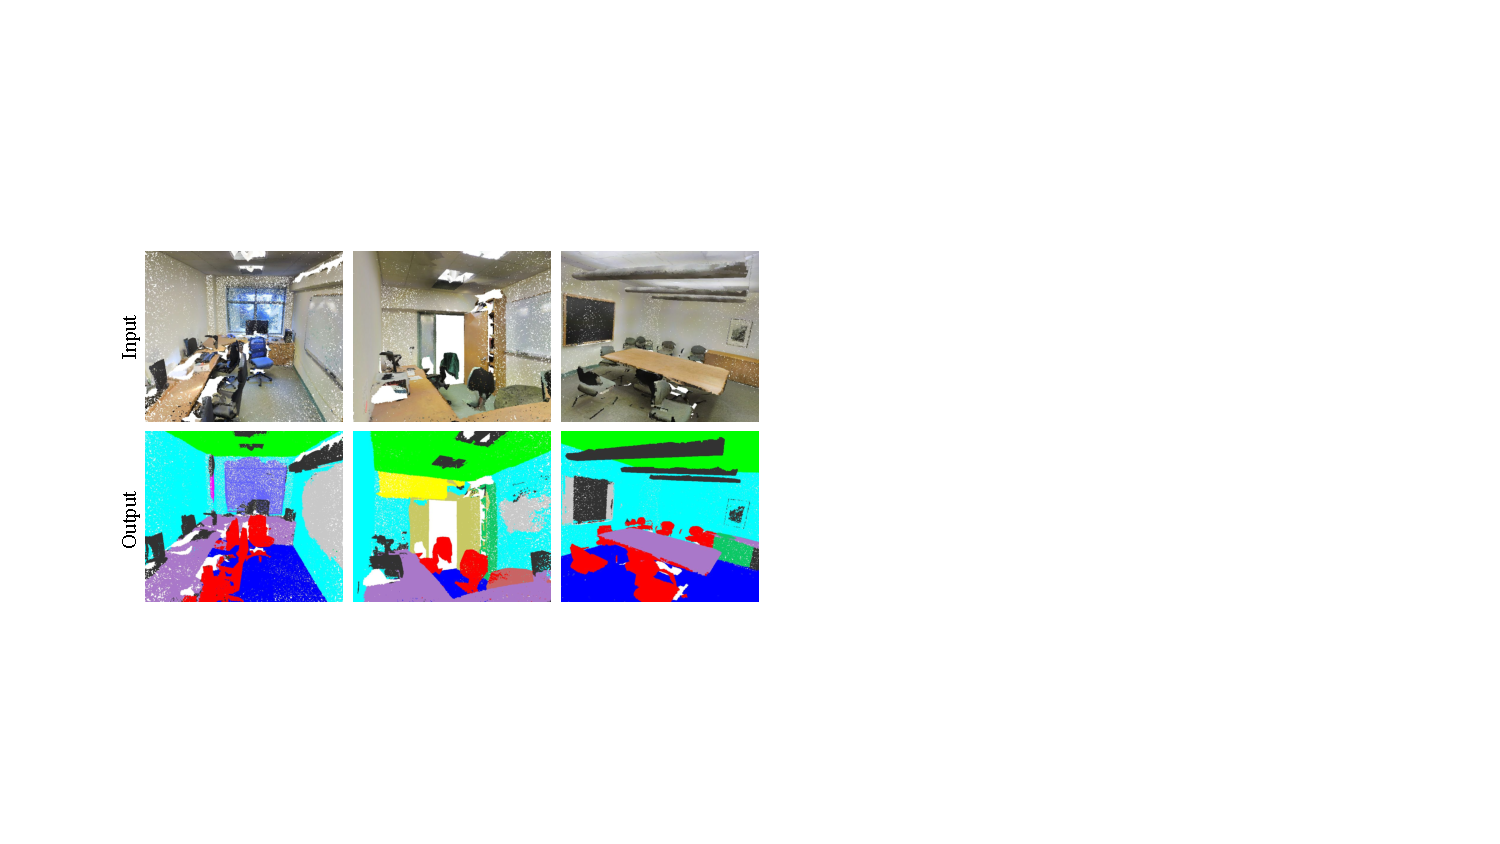
\includegraphics[width=0.8\linewidth,height=4cm]{fig/semantic}
    \caption{\textbf{语义分割的定性结果} 上一行是带颜色纹理的点云。底下是输出的语义分割结果(以点云展示),输出结果展示同输入的相机角度一致。}
    \label{fig:qualitative_segmentation}
\end{figure}

\subsection{架构设计分析}
\label{sec:arch_analysis}

在本节中,我们通过控制验证我们的设计选择实验。我们还展示了我们网络超参数的影响。
%~\footnote{Due to the limit of space, we refer the analysis on bottleneck dimension and number of input points to supplementary.}


\paragraph{与替代顺序不变方法的比较} 如第~\ref{sec:pointnet_arch}节所述,至少有三种选择可用于使用无序集合输入。我们使用ModelNet40形状分类问题作为测试平台来比较这些选项,以下两个控制实验也将使用此任务。

我们比较的基准线 (如图~\ref{fig:order_invariant}所示)包括:未排序和已排序的 $n \times 3$ 数组的多层感知机,将输入点视为序列的RNN模型,以及基于对称函数的模型。我们实验的对称操作包括最大池化、平均池化和基于注意力的加权和。注意方法类似于~\cite{vinyals2015order}中的方法,即从每个点特征预测一个标量分数,然后通过计算softmax跨点对分数进行归一化。然后根据归一化分数和点特征计算加权和。如图~\ref{fig:order_invariant}所示,最大池化操作以较大的优势幅度实现了最佳性能,这验证了我们的选择。


% \begin{table}
%     \small
%     \centering
%     \begin{tabular}[width=\linewidth]{l|c}
%     \hline
%     ~                    & accuracy \\ \hline
%     MLP (unsorted input) & 24.2       \\
%     MLP (sorted input)   & 45.0       \\
%     LSTM                 & 78.5       \\ \hline
%     Attention sum        & 83.0       \\
%     Average pooling      & 83.8       \\
%     Max pooling          & \textbf{87.1}       \\ \hline
%     \end{tabular}
%     \caption{\textbf{Comparing different order invariant methods.} Metric is classification overall accuracy on ModelNet40 test set. Max pooling is performing surprisingly well.}
%     \label{tab:order_invariant}
% \end{table}

\begin{figure}[t!]
    \centering
    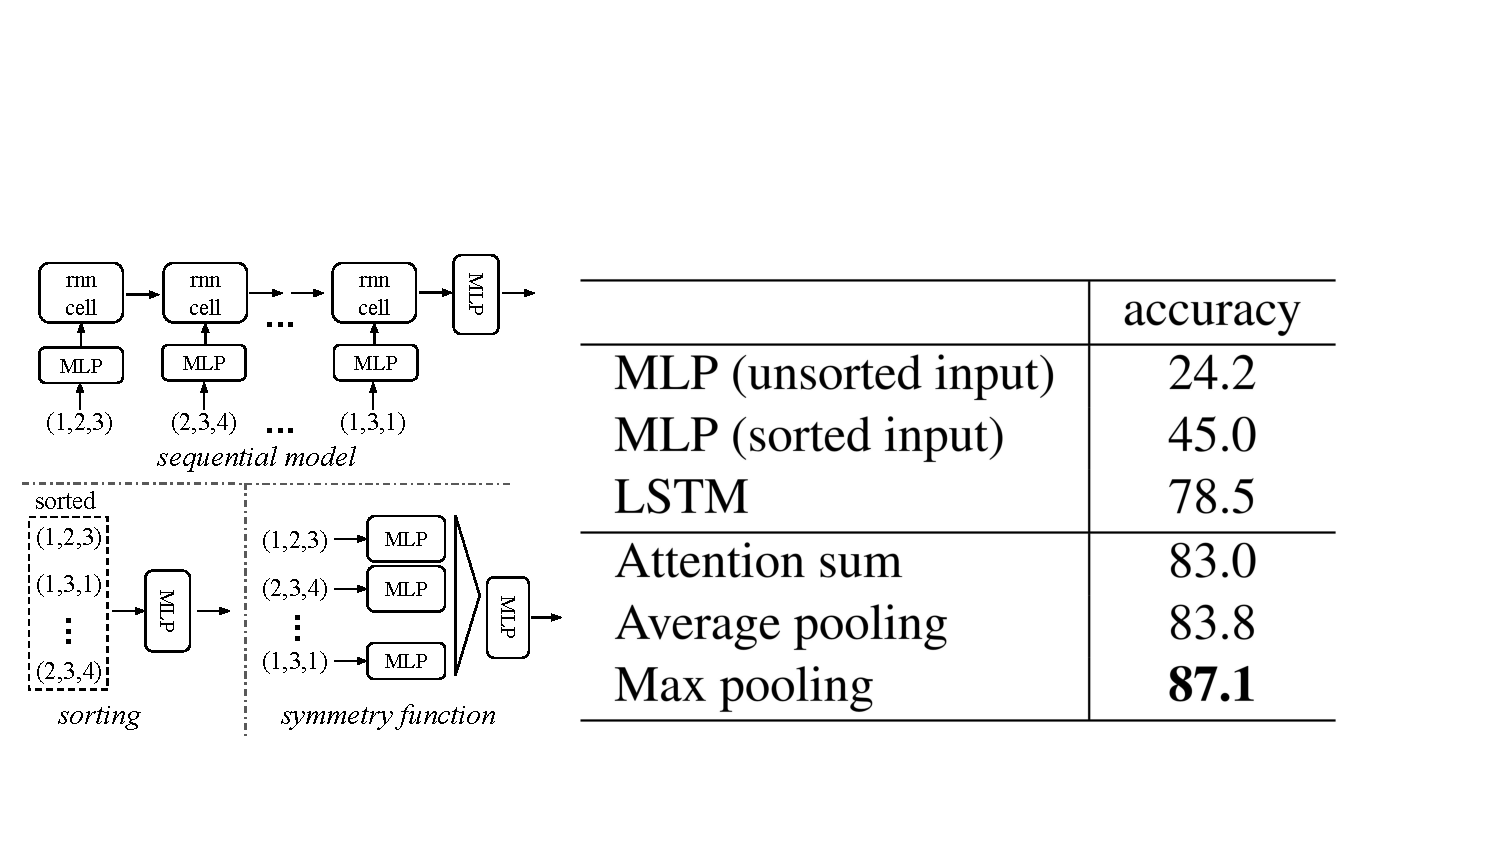
\includegraphics[width=\linewidth]{fig/order_invariant2.pdf}
    \caption{\textbf{三种实现顺序不变性的方法}神经元尺寸为64,64,64,128,1024,的5层隐藏层的多层感知机(MLP)应用在点集上,所有点共享一个简单的MLP副本。靠近输出的MLP共有两层,尺寸为512,256。}
    \label{fig:order_invariant}
\end{figure}

\paragraph{输入和特征转换的有效性} 在表~\ref{tab:transform}中,我们展示了我们的输入和特征转换(用于对齐)的积极影响。有趣的是,最基本的架构已经取得了相当合理的结果。使用输入转换可提高 $0.8\%$ 的性能。正则化损失是高维变换起作用所必需的。通过结合转换和正则化项,我们实现了最佳性能。

\begin{table}[b!]
    \small
    \centering
    \begin{tabular}[width=\linewidth]{l|c}
    \hline
    Transform              & accuracy \\ \hline
    none                   & 87.1     \\ \hline
    input (3x3)            & 87.9     \\
    feature (64x64)        & 86.9     \\
    feature (64x64) + reg. & 87.4     \\ \hline
    both                   & \textbf{89.2}     \\ \hline
    \end{tabular}
    \caption{\textbf{输入特征转换的效果} 评价指标是ModelNet40测试集上的总体分类准确率}
    \label{tab:transform}
\end{table}


% \paragraph{Effects of Max Layer Size and Number of Points} Here we show our model's performance change with regard to the size of the first max layer output as well as the number of input points. In Fig~\ref{fig:net_param} we see that performance grows as we increase the number of points however it saturates at around 1K points. The max layer size plays an important role, increasing the layer size from 64 to 1024 results in a $2-4\%$ performance gain. It indicates that we need enough point feature functions to cover the 3D space in order to discriminate different shapes.

% \begin{figure}
%     \centering
%     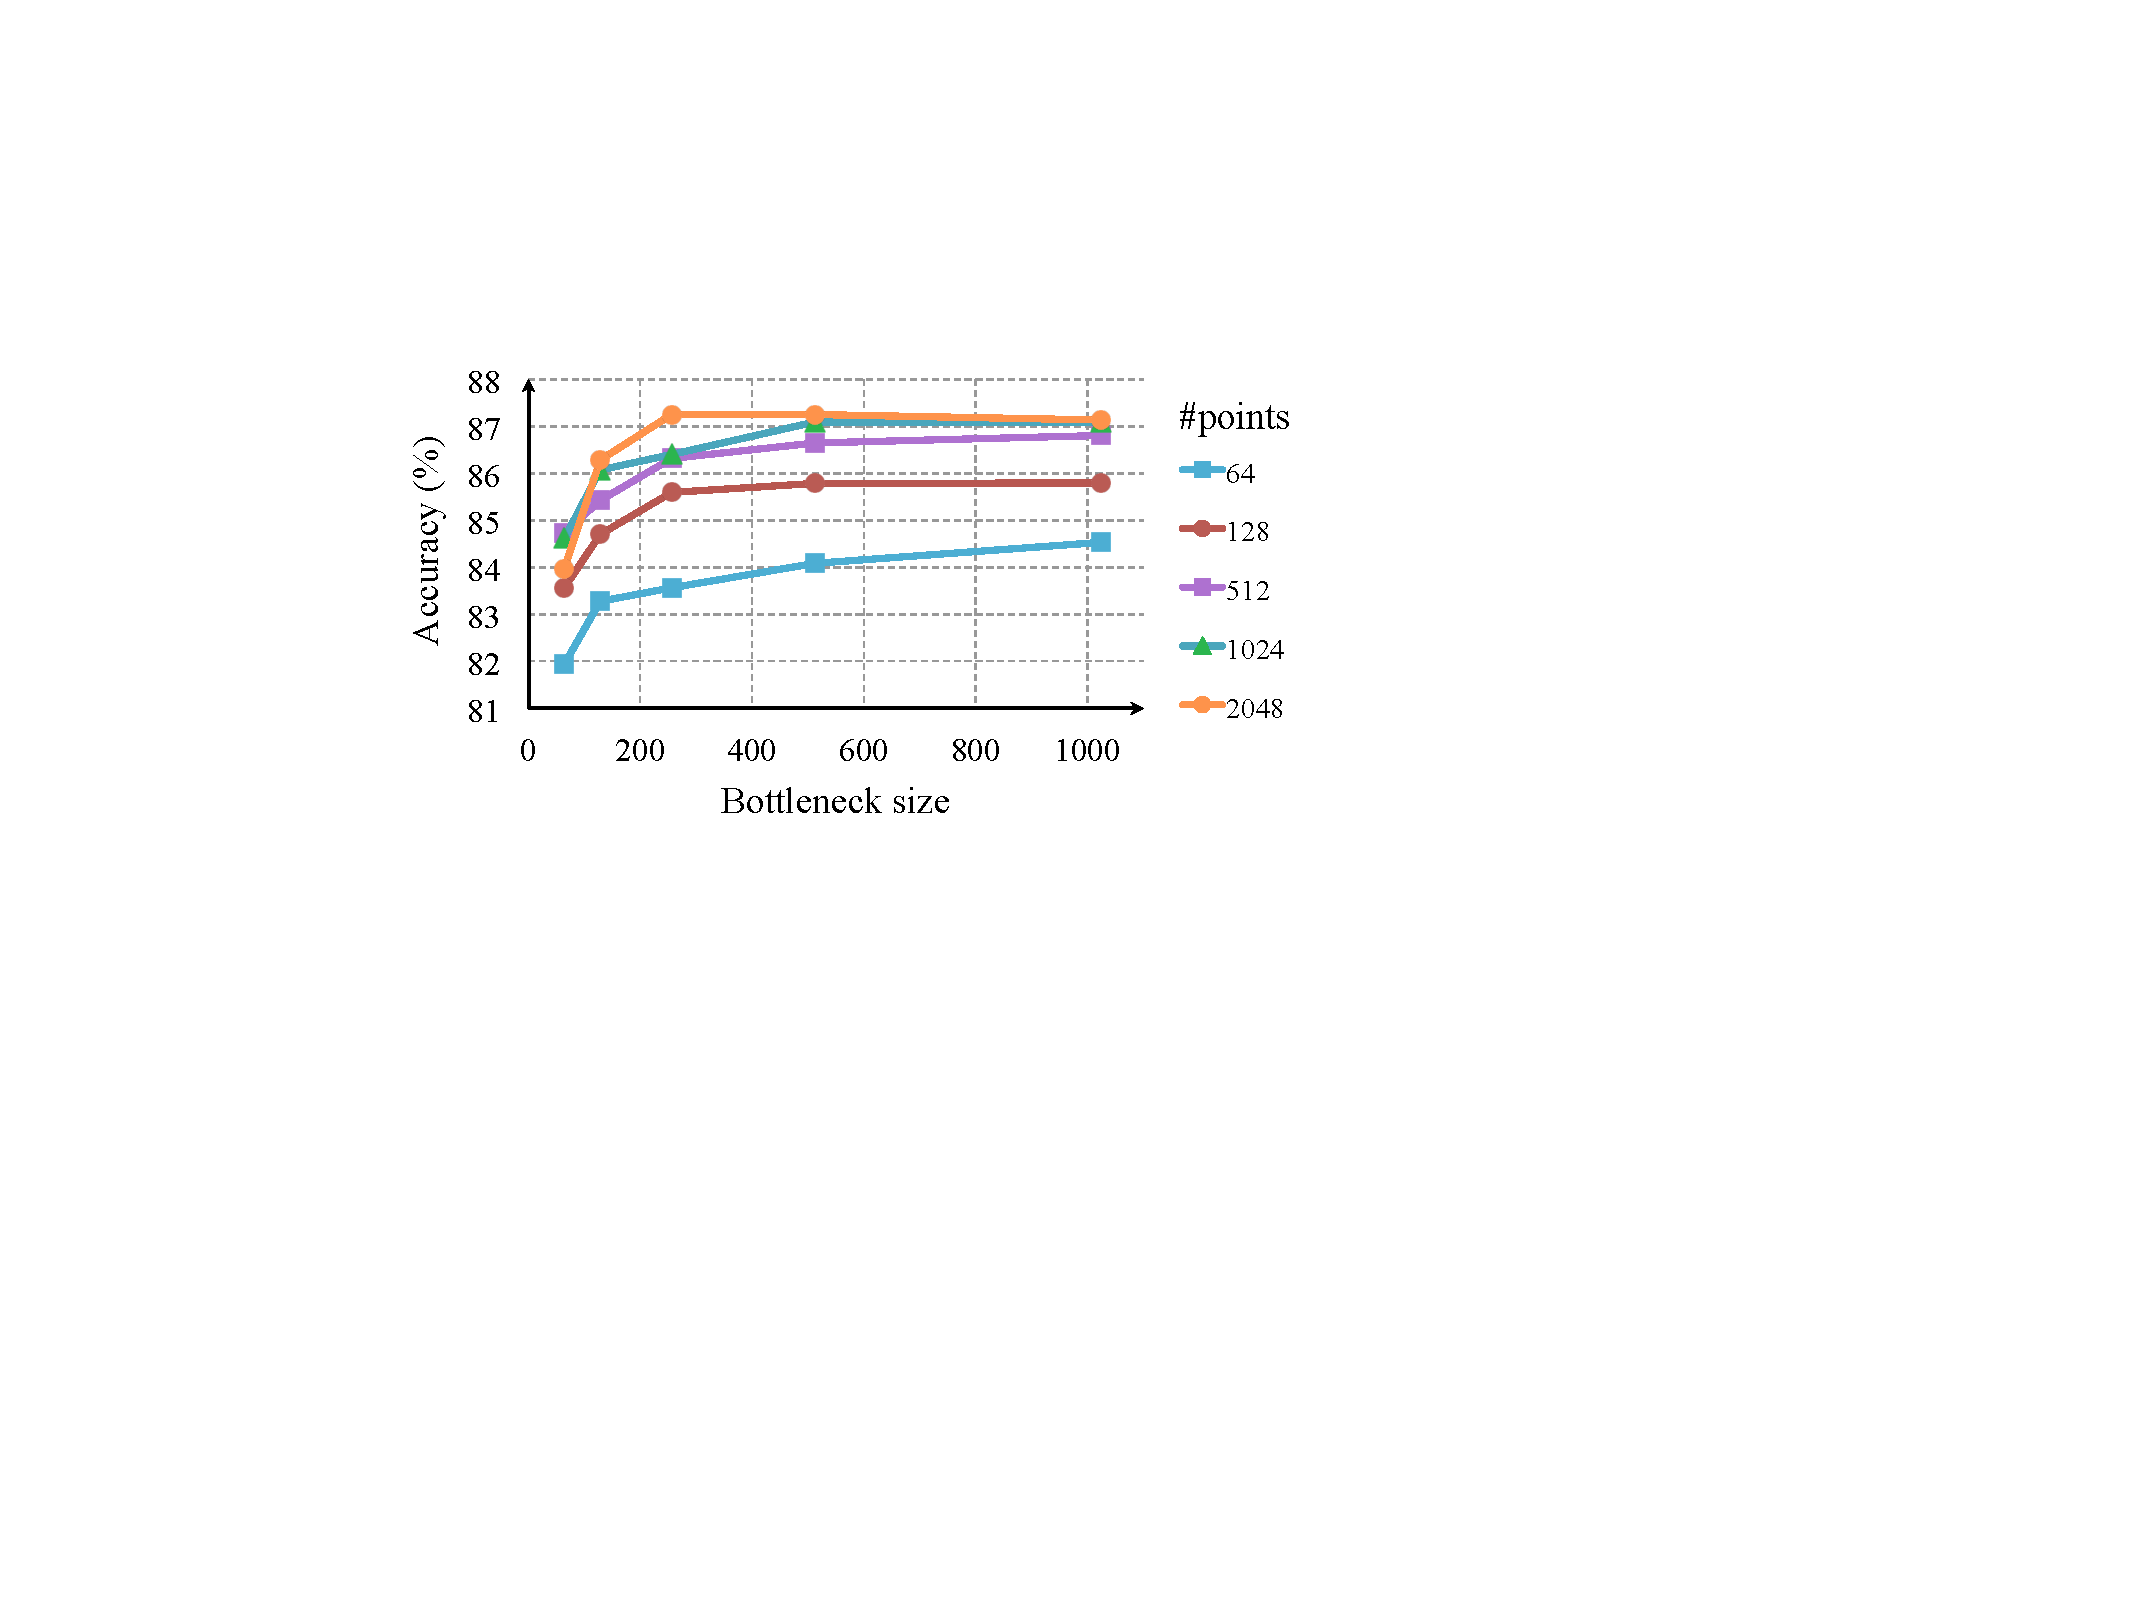
\includegraphics[width=0.8\linewidth]{fig/bottleneck.pdf}
%     \caption{\textbf{Effects of bottleneck size and number of input points.} The metric is overall classification accuracy on ModelNet40 test set.}
%     \label{fig:net_param}
% \end{figure}

\paragraph{鲁棒性测试} 我们展示了我们的PointNet不仅简单有效,还对各种输入损坏具有鲁棒性。我们使用与图~\ref{fig:order_invariant}的最大池化网络相同的架构。输入点被归一化为一个单位球体。结果如图~\ref{fig:robustness}。

A对于缺失点,当有 $50\%$ 的点缺失时,准确率仅下降 $2.4\%$ ,并且对于最远和随机输入采样则是 $3.8\%$ 。我们的网络在训练期间看到了异常点你,那么它对异常点也具有鲁棒性,。我们评估了两种模型:一种在具有 $(x,y,z)$ 坐标的点上进行训练;另一个在 $(x,y,z)$ 上加上点密度。即使当 $20\%$ 的点是异常值,网络也有超过 $80\%$ 的准确率。图~\ref{fig:robustness}右侧显示了网络对点扰动的鲁棒性。

\begin{figure}
    \centering
    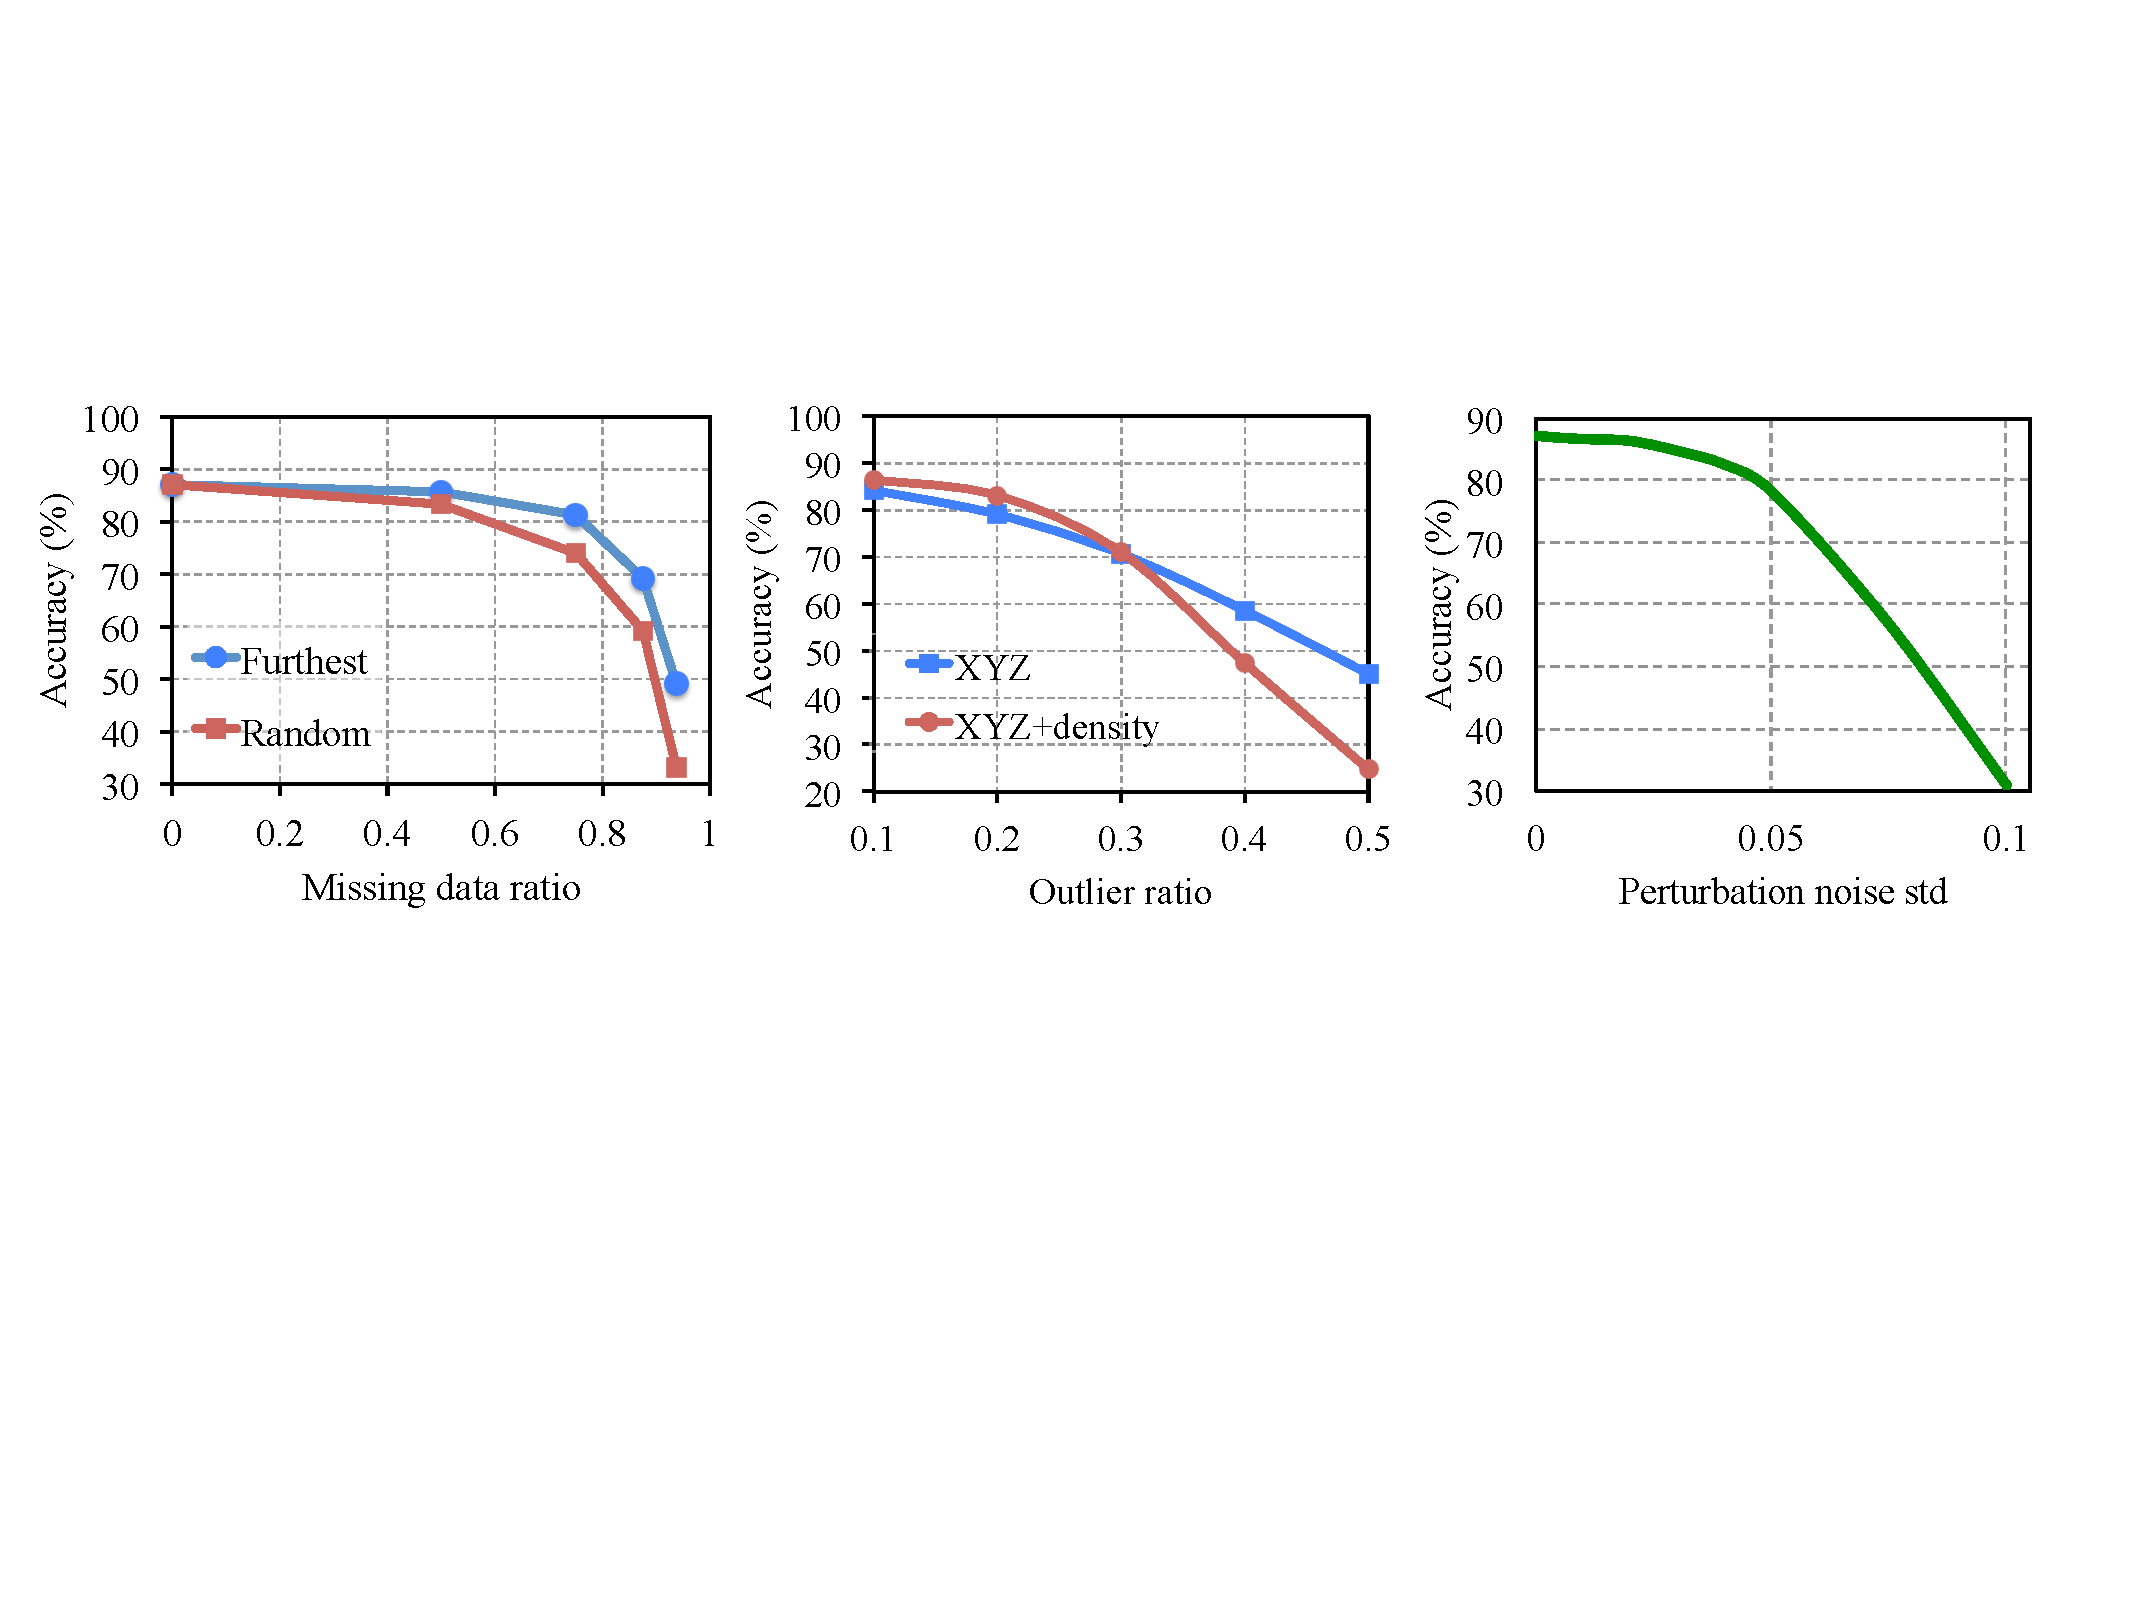
\includegraphics[width=\linewidth]{fig/robustness.pdf}
    \caption{\textbf{PointNet鲁棒性测试} 评价指标是ModelNet40测试集上的总体分类准确率。 左侧: 删除点的情况 Furthest意思是对1024个原始点采用最远点采样。 中间: 离群点插入的情况。离群点均匀的分布在单位球体中。 右侧: 点扰动的情况。单独对每个点进行高斯噪声扰动}
    \label{fig:robustness}
\end{figure}

\begin{comment}
\paragraph{MNIST Digit Classification} While we focus on 3D point cloud learning, a sanity check experiment is to apply our network on a 2D point clouds - pixel sets.

To convert an MNIST image into a 2D point set we threshold pixel values and add the pixel (represented as a point with XY coordinate in the image) with values larger than 128 to the set. We use a set size of 256. If there are more than 256 pixels int he set, we randomly subsample it; if there are less, we pad the set with the one of the pixels in the set (due to our max operation, which point used for the padding will not affect outcome). 
3
As seen in Table~\ref{tab:mnist}, we compare with a few baselines including multi-layer perceptron that considers input image as an ordered vector, a RNN that consider input as sequence from pixel (0,0) to pixel (27,27), and a vanila CNN. It's interesting to see that our model can achieve quite good performance by considering the image as a 2D point set.

% vanila CNN: https://www.microsoft.com/en-us/research/publication/best-practices-for-convolutional-neural-networks-applied-to-visual-document-analysis/
\begin{table}[h!]
    \centering
    \begin{tabular}[width=\linewidth]{l|c|c}
    \hline
    ~                      & input & error (\%) \\ \hline
    Multi-layer perceptron~\cite{simard2003best} & vector & 1.60  \\
    LeNet5~\cite{lecun1998gradient}                 & image & 0.80 \\ \hline
    Ours PointNet          & point set & 0.78 \\ \hline
    \end{tabular}
    \caption{\textbf{MNIST classification results.} We compare with vanila versions of other deep architectures to show that our network based on point sets input is achieving reasonable performance on this traditional task.}
    \label{tab:mnist}
\end{table}
\end{comment}


% \begin{figure}[b!]
%     \centering
%     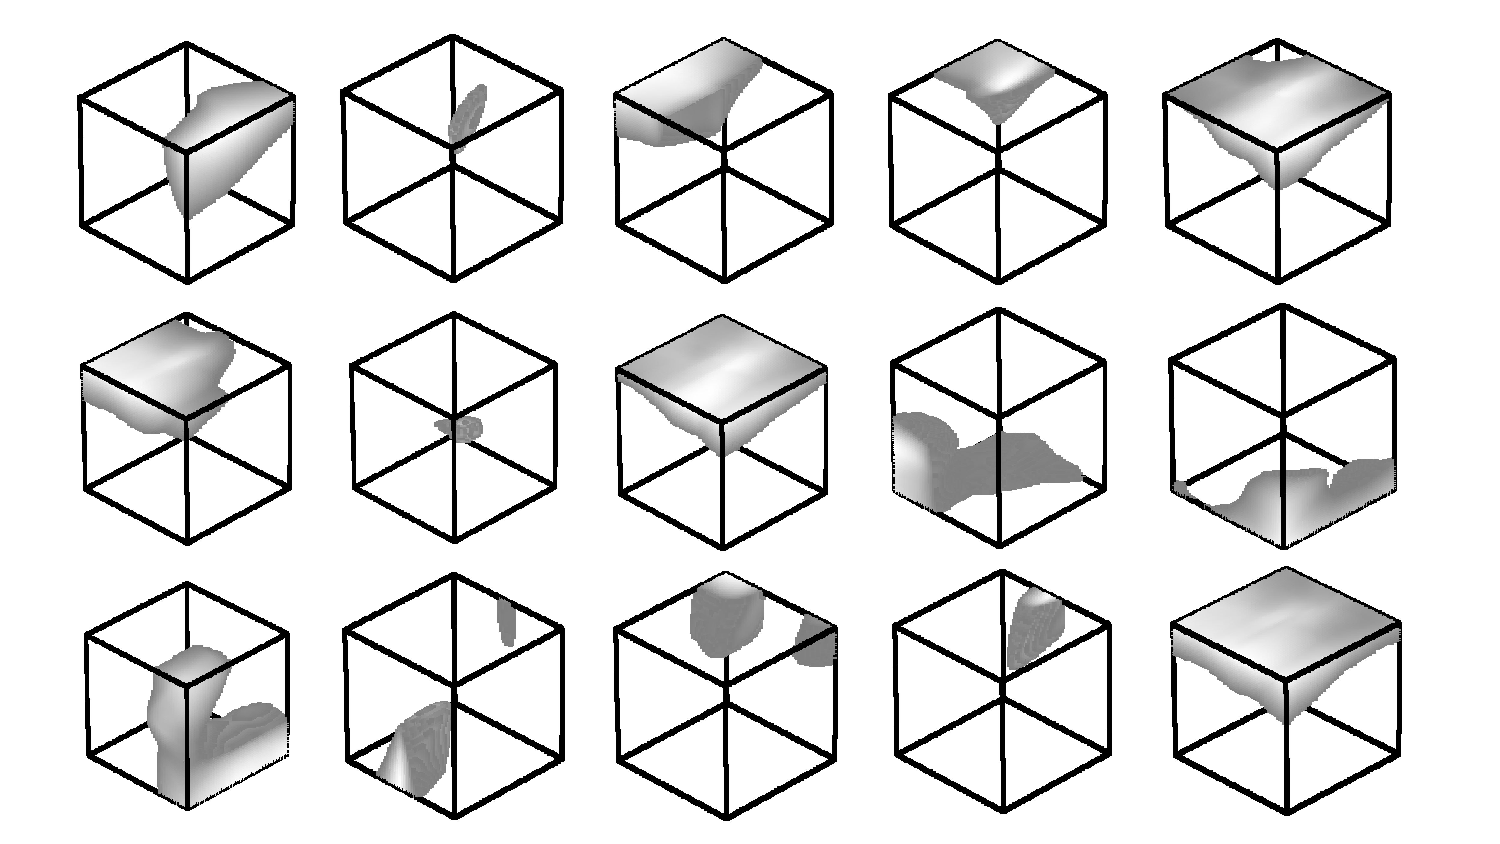
\includegraphics[width=0.7\linewidth]{fig/kernels.pdf}
%     \caption{\textbf{Point function visualization.} For each per-point function $h$, we calculate the values $h(p)$ for all the points $p$ in a cube of diameter two located at the origin, which spatially covers the unit sphere to which our input shapes are normalized when training our PointNet. In this figure, we visualize all the points $p$ that give $h(p)>0.5$ with function values color-coded by the brightness of the voxel. We randomly pick 15 point functions and visualize the activation regions for them.}
%     \label{fig:functions}
% \end{figure}


\subsection{可视化PointNet}
\label{sec:visualizing_pointnet}
% We design two experiments to visualize what has been learnt by the PointNet. The results are consistent with the theoretical analysis in Sec~\ref{sec:theory}. In the first experiment, we visualize the learnt point function $h(x)$ in Eq~\ref{eq:approx}, which demonstrates that our network learns a family of optimization criteria that selects informative points from the cloud. Our second experiment illustrates the robustness of our network, as explained in Thm~\ref{thm:thm2}.

% \paragraph{Point Function Visualization} As discussed in Sec~\ref{sec:pointnet_arch}, our network computes $K$ (we take $K=1024$ in this experiment) dimension point features for each point and aggregates all the per-point local features via a max pooling layer into a single $K$-dim vector, which forms the global shape descriptor. 

% To gain more insights on what the learnt per-point functions $h$'s detect, we visualize the points $p_i$'s that give high per-point function value $f(p_i)$ in Fig~\ref{fig:functions}. This visualization clearly shows that different point functions learn to detect for points in different regions with various shapes scattered in the whole space. 

\begin{comment}
This visualization is similar to the kernel visualization in convolutional neural networks in the sense that we'd like to know what input patterns would activate a specific neuron. However, our point function is behaving in a very differnt way from conv kernels.
\end{comment}

在图~\ref{fig:recon},我们可视化了一些样本形状 $S$ 的 \textit{关键点集} $\mathcal{C}_S$ 和 \textit{上边界形状} $\mathcal{N}_S$ (如Thm~\ref{thm:thm2}所述)。两个形状之间的点集将给出完全相同的全局形状特征 $f(S)$。

从图~\ref{fig:recon} 可以清楚地看出, \textit{关键点集} $\mathcal{C}_S$中对最大池化特征有贡献的点,总结了形状的主干。
%, or sample a sparse collection of points to describe the geometry of the whole shape.
\textit{上界形状} $\mathcal{N}_S$ 说明了与输入点云 $S$ 具有相同全局形状特征 $f(S)$ 的最大可能点云。$\mathcal{C}_S$ 和 $\mathcal{N}_S$反映了PointNet的鲁棒性,这意味着丢失一些非关键点不会改变全局形状特征 $f(S)$。



% We visualize the shape family, as discussed in Thm~\ref{thm:thm2}, including all the shapes between the \textit{critical point set} $\mathcal{C}_S$ and the \textit{upper-bound shape} $\mathcal{N}_S$ that gives the same global feature $f(S)$ with respect to a given shape $S$.

\begin{figure}[b]
    \centering
    % \includegraphics[width=0.8\linewidth]{fig/recon.pdf}
    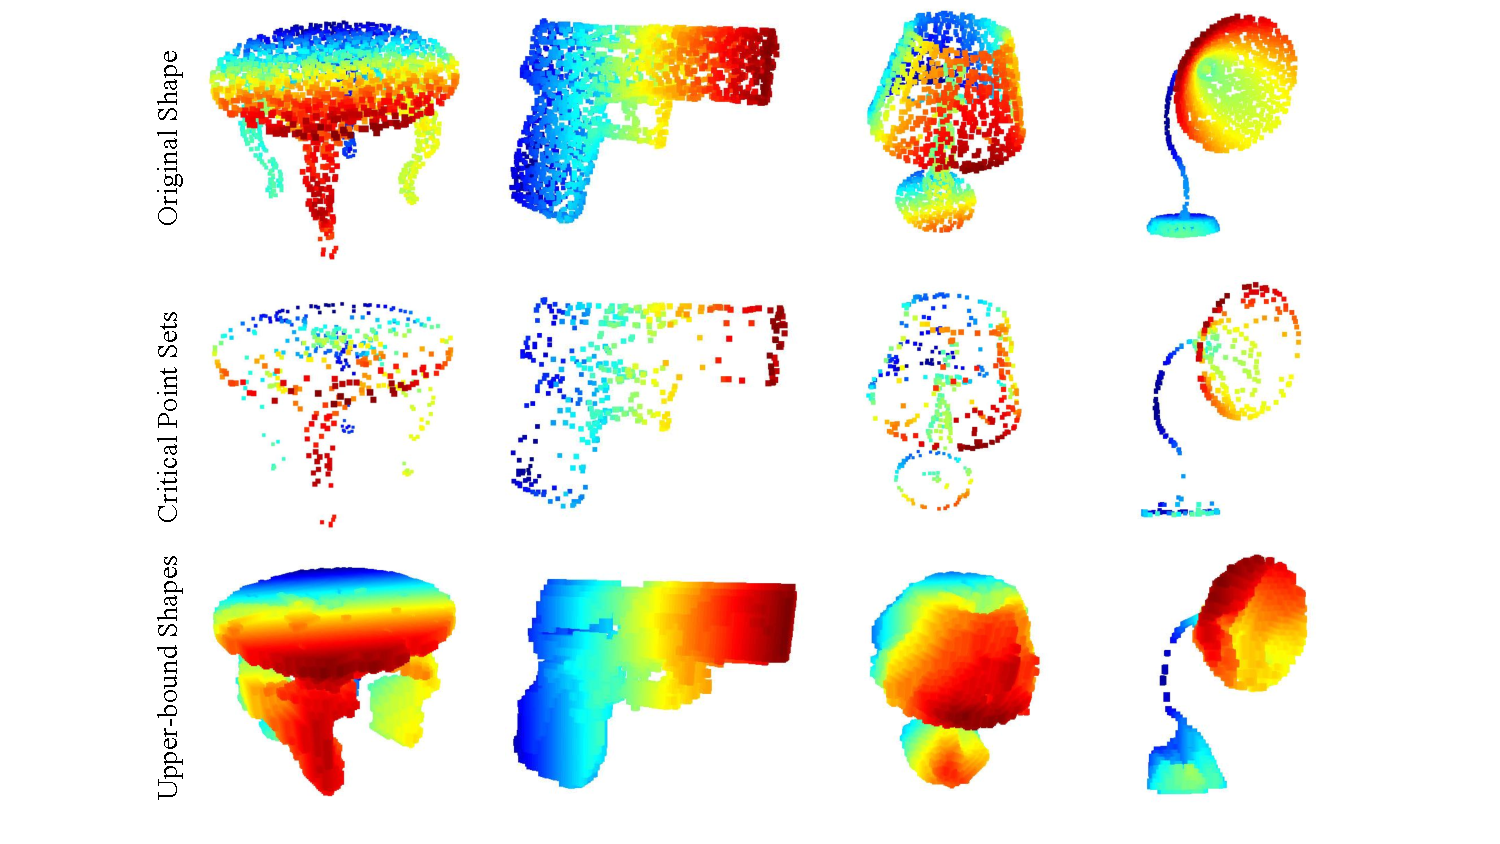
\includegraphics[width=0.8\linewidth]{fig/kp_ss_visu1.pdf}
    \caption{\textbf{关键点集和上界形状} 关键点集和上界形状共同决定了给定形状的全局形状特征,任何处于关键点集和上界形状间的点云都有同样一致的特征。 我们通过色彩编码来体现物体的深度信息。}
    \label{fig:recon}
\end{figure}

% Fig~\ref{fig:recon} shows the \textit{critical point sets} $\mathcal{C}_S$ and \textit{upper-bound shapes} $\mathcal{N}_S$ for four selected shapes. 
%The original input point clouds are rendered in the first row while the $\mathcal{C}_S$ and $\mathcal{N}_S$ for them are shown in the second and their rows respectively.
%The $\mathcal{C}_S$ for a given shape $S$ includes the points from the original point cloud that activates some point function $h_i$'s the most. 
$\mathcal{N}_S$ 是通过将边长为2的立方体中的所有点经过网络前向传播后,选择点函数值$(h_1(p), h_2(p), \cdots, h_K(p))$ 不大于全局形状描述符的点 $p$ 来构建的。
% It is not hard to see that all the shapes $S'$ that cover $\mathcal{C}_S$ and are contained by $\mathcal{N}_S$ give the exactly same global feature $f(S')=f(S)$. The transition shape family entails the robustness of the our PointNet, meaning that adding noisy jitterings or losing some non-critical points do not change the learnt shape signature and thus do not affect our classification or segmentation results.

\begin{comment}
We start from a max pooled vector of a specific input point cloud $X$, and find a set of point cloud $S$ (it's a set of point sets) where each point cloud in the set $S$ will result in the same max pooled vector as to $X$. In another word, we will reconstruct the input with only the knowledge of $X$ and the network parameters.

Assuming when feeding input point cloud $X$ to the network the first max-pooling layer's output is $g(X) = MAX\{f(x_1), f(x_2), ..., f(x_N)\} \in \R^{1024}$, where $X = \{x_1, x_2, ..., x_N\}$. We achieve the reconstruction by firstly construct a dense volumetric grids. Each voxel represents a point in 3D space. Then we will sweep through each point $p$ in the volume and judge whether this point's feature $f(p) \in \R^{1024}$ has any value larger than that in the corresponding dimension of $g(X)$. If there is , it means the point $p$ cannot be the input that results in $g(X)$, so we will exclude this point. After sweeping the volume, all the points left are possible to be part of the input set $X$. This set of points forms a upper bound of any possible input set that gets max pooling outcome of $g(X)$. Some reconstructed results of this upper bound is visualized in the second row of Fig~\ref{fig:recon}.

On the other hand, if we know the input set (set $X$) and the network, we can know which input points (subset $Y$ of $X$) are actually contributing to the final value of the max pooled vector. Excluding all the points in $X \\ Y$ will not affect the result. We call this contributing set of points the lower bound of the input, as visualized in the third row of Fig~\ref{fig:recon}. Any point sets that fall between the lower bound and upper bound will result in exactly the same result.
\end{comment}





\subsection{时间和空间复杂度分析}
\label{sec:complexity}
表~\ref{pointnet_complexity} 总结了我们PointNet分类网络的空间(网络中的参数个数)和时间(浮点运算/样本)复杂性。我们还将PointNet与之前工作中的一组具有代表性的基于体积和多视图的架构进行了比较。

尽管MVCNN~\cite{su15mvcnn} 和Subvolume (3D CNN) ~\cite{qi2016volumetric} 实现了高性能,PointNet的计算成本更低,效率更高(以FLOPs/样本衡量:效率分别提高\emph{141倍} 和 \emph{8倍})。此外,就网络中的\#param(参数少\emph{17倍})而言,PointNet的空间效率比MVCNN高得多。此外,PointNet更具可扩展性——它的空间和时间复杂度为 $O(N)$ —— 与输入点的数量呈\emph{线性} 关系。然而,由于卷积占用计算时间,多视图方法的时间复杂度随图像分辨率\emph{平方级}增长,基于体积卷积的方法随着体积大小成\emph{立方级}增长。

根据经验,PointNet能够处理超过每秒100万个点用于点云分类(约1K对象/秒)或语义分割(约2个房间/秒),在TensorFlow上使用1080XGPU,显示出实时应用的巨大潜力。

\begin{table}[h!]
    \centering
    \begin{tabular}{|l|l|l|l|}
    \hline
    ~                & \#params & FLOPs/sample\\ \hline
    PointNet (vanilla)  & 0.8M                        & 148M \\
    PointNet         & 3.5M                         & 440M \\ \hline
    %VoxNet~\cite{maturana2015voxnet}           & 0.07M                        & 204M \\
    Subvolume~\cite{qi2016volumetric} & 16.6M                        & 3633M \\ \hline
    MVCNN~\cite{su15mvcnn}   & 60.0M                          & 62057M \\ \hline
    \end{tabular}
    \caption{\textbf{处理3D数据分类的深度学习架构的时间和空间复杂度} PointNet (vanilla) 是分类版的PointNet除去输入和特征转化部分的版本。 FLOP代表浮点运算操作。
    ``M'' 代表百万。 Subvolume和MVCNN都使用了多次旋转和多个视角池化后的数据,没有这些操作他们的表现会大大下降}
    \label{pointnet_complexity}
    \vspace{-3mm}
\end{table}